\chapter{Wstęp teoretyczny}
\label{cha:wstepTeoretyczny}

%---------------------------------------------------------------------------

\section{Procesy biznesowe}
\label{sec:procesyBiznesowe}

\subsection{Procesy biznesowe}
W każdym dużym przedsiębiorstwie, każdego dnia, wykonywana jest ogromna ilość czynności koniecznych do funkcjonowania tej organizacji. Ludzie oraz oraz systemy podejmują najróżniejsze działania związane z różnymi, często nie mającymi wiele wspólnego zadaniami. Mogą to być działania jak obsługa płatności, obsługa zamówień, wytwarzanie produktów czy ich transport. Przykłady te można mnożyć w zależności od sektora w jakim obraca się dana firma. Im jest ona większa, tym trudniej jest osobom zarządzającym opisać czy zrozumieć poszczególne czynności. W pewnym momencie, kiedy ilość rożnych zadań rośnie do setek czy tysięcy staje się to niemożliwe i potrzebny jest sposób na zebranie wiedzy o pojedynczych operacjach i opisanie jej za pomocą uporządkowanej struktury. Stąd narodził się pomysł na wykorzystanie wykorzystanie procesów biznesowych.

Procesy biznesowe opisują zbiór aktywność, które podejmuje grupa podmiotów w celu osiągnięcia celu biznesowego. W literaturze brakuje jednej ogólnie przyjętej definicji procesu biznesowego. W latach 90. XX wieku proponenci BPR, czyli Przeprojektowania procesów biznesowych (\textit{eng. Business process re-engineering}) starali się sprecyzować pojęcie procesu biznesowego. W książce "Process Innovation: Reengineering Work through Information Technology"\cite{davenport1993process} Davenport określił termin ten jako "Ustrukturyzowany, mierzalny zbiór działań, których celem jest wytworzenie określonego produktu dla określonego klienta lub rynku". Autor położył nacisk na zbiór kroków prowadzących do celu, raczej niż na końcowy efekt. W dalszej części autor pisze "Proces jest zatem określonym uporządkowaniem czynności roboczych w czasie i przestrzeni, z początkiem i końcem oraz jasno określonymi wejściami i wyjściami: strukturą działania.". Inni pionierzy BPR Michael Hammer i James Champy proponują podejście „Proces biznesowy to zbiór działań, który pobiera jeden lub więcej rodzajów danych wejściowych i tworzy wynik, który ma wartość dla klienta”\cite{HAMMER199390}. Autorzy dają większą dowolność, co do definicji procesu, nie wspominając o konieczności jego logicznej organizacji czy mierzalności. Z kolei Jacobson zupełnie pomija konieczność zamknięcia procesu w jakiekolwiek ramy: "Zestaw czynności wewnętrznych wykonywanych w celu obsługi klienta"\cite{JacobsonObjectAdvantage}. Nacisk na konieczność odniesienia procesów do wymiernych środków firmy widzimy w definicji: "Procesy biznesowe są aktywną częścią biznesu. Opisują funkcje firmy i obejmują zasoby, które są używane, przekształcane lub wytwarzane. Proces biznesowy to abstrakcja, która pokazuje współpracę między zasobami i transformację zasobów w biznesie. Podkreśla, w jaki sposób wykonywana jest praca, zamiast opisywać produkty lub usługi wynikające z tego procesu."\cite{Eriksson2000BusinessMW}. Szczególnie ważny jest tutaj fragment o transformacji zasobów, gdyż każe on rozumieć poszczególne aktywności w procesie jako powiązane ze sobą i kończące się namacalnymi rezultatami. Definicja "Proces biznesowy to seria kroków mających na celu wytworzenie produktu lub usługi. W wyniku niektórych procesów produkt lub usługa jest odbierana przez zewnętrznego klienta organizacji. Nazywamy te podstawowe procesy. Inne procesy wytwarzają produkty, które są niewidoczne dla klienta zewnętrznego, ale są niezbędne do efektywnego zarządzania firmą. Nazywamy te procesy wsparcia"\cite{rummler_brache_1995} wprowadza rozgraniczenie na podtypy procesów. Ważnym jest jednak że nie jest koniecznością, aby rezultaty procesu były widoczne na zewnątrz organizacji.  

Powyższe definicji skupiają się na delikatnie odmienny aspektach procesów biznesowych, nie zawsze szczegółowo wspominając o innych. Starając się usystematyzować powyższe sformułowania, chcąc zbudować bazę do dalszej analizy tematu, można przyjąć, że procesy biznesowe charakteryzują:
\begin{itemize}
  \item[•] Określony cel, którym jest wytworzenie wartości dla klienta zewnętrznego lub pośrednio firmy - klienta wewnętrznego. Jednak warto jeszcze raz zaznaczyć ze proces biznesowy skupia się na sposobie osiągnięcia celu, a nie opisie celu samego w sobie. 
  \item[•] Dyskretny, jasno zdefiniowany i identyfikowalny zbiór aktywności. 
  \item[•] Jasno określony początek - wejście i koniec - wyjście.
  \item[•] Pomiędzy kolejnymi procesami zachodzi zależność przyczynowo-skutkowa.
\end{itemize}

Żeby lepiej zilustrować czym jest proces biznesowy, poniżej znajduje się prosty przykład często spotykanego procesu. Oczywiście, prawdziwy proces będzie posiadał o wiele więcej aktywności.

\begin{figure}[h]
	\centering{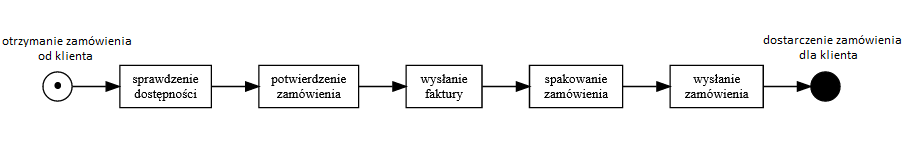
\includegraphics[scale=0.7]{simple-business-process.png}}
	\caption{\label{fig:subcaption_example}Przykład prostego procesu}
\end{figure}

Zauważmy, że mamy jasno zdefiniowany wejście - otrzymanie zamówienia od klienta oraz wyjście, kiedy dostarczamy oczekiwaną wartość dla klienta, a całość składa się z serii tworzących logiczną całość aktywności. Aktywności są konkretnie zdefiniowane. Standardem jest definiowanie aktywności w formie równoważników zdań.


\subsection{Zarządzanie procesami biznesowymi}
Zdefiniowanie proces biznesowego otwiera wiele możliwości analizy działań przedsiębiorstwa i w skutek tego wprowadzanie usprawnień. Dziedziną, która się tym zajmuje jest zarządzanie procesami biznesowymi (\textit{eng. Business process modeling}) zwane w skrócie BPM jest dziedziną. Sercem jest proces, a sam BPM może określić jako zbiór metod, technik i sposobów służący do projektowania, wprowadzania w życie, zarządzania i analizy procesów biznesowych\cite{BPMDemystified}. 

Celem stosowania metod zarządzanie procesami biznesowym jest 
Metoda te są obecnie szeroko stosowane przez organizacje i uznawane za arcyważną składową sukcesu danego podmiotu. 
Ważny jest człowiek
W publikacji \cite{SixElementsBPM} wyróżniono 6 podstawowych elementów BPM. Są to dopasowanie strategiczne, zarządzanie, modelowanie, techniki informatyczne, ludzie, kultura. Cześć z tych elemetów jest niezbyt ściśle zdefiniowiowane i wymaga bardziej ogólnego podejście, jednak do części z nich można z pomyślnością zastosować metody informatyczne. I dlatego to i to zaczęło czerpać ze zdobyczy informatyki
\cite{BPMWhat}
Business process lifecycle
W dalszej cześci pracy przedstawione zostaną sposoby na wykorzystanie d
%---------------------------------------------------------------------------

\section{Modelowanie procesów biznesowych}
\label{sec:modelowanie}
\subsection{Notacja}
Najpopularniejszą notacją używaną do opisu procesów biznesowych jest BPMN. 
W tutajbadanie opisano najpopularniejsze elementy używane w BPMN. 
\subsection{Modelowanie procesów biznesowych}
Przyjrzyjmy się sytuacji, w której klient chce naprawić pralkę. Klient initializuje proces naprawy kontaktując się z firmą naprawiającą sprzęt AGD. Rezulty tego procesu mogą być 2 : naprawiona i nie, a sam proces może się wykonać na duża ilość sposobów, to sprawia, że proces rośnie i potrzebne są metoda na uporządkowanie tego procesu w celu chociażby zwiększenia wydajności.

Grafika skomplikowanego procesu

Jest to szeroko pojęta dziadzina, która zawiera różne aplikacje metoda informatyki do procesów. 
Wyróżnia 3 podkategorie: odkrywanie, conformance checking 
Odkrywanie procesów
Metryki ważne

\subsection{Dzienniki zdarzeń}

\begin{figure}[h]
	\centering{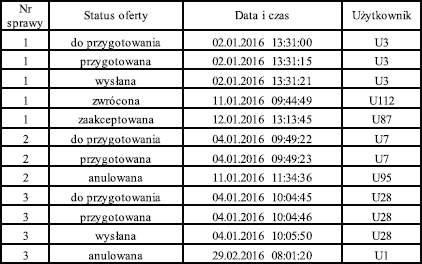
\includegraphics[scale=0.8]{event-log.png}}
	\caption{\label{fig:subcaption_example}Przykład dziennika zdarzeń}
\end{figure}s

W kontekście odkrywania procesów biznesowych ważne są dla nas tylko zdarzenia i kolejność ich wykonywania. Informacje o dokładnym czasie wykonania oraz użytkowniku, który wykonał daną operację możemy pominąć. Ponadto musimy wiedzieć jak często dany wariant wystąpił.

\subsection{Odkrywanie procesów biznesowych}

Odkrywanie procesów biznesowy jest podgrupą i obejmuję techniki przekształcania danych w procesy.
Procesy zaprojektowane nie zawsze są realizowane w praktyce. Ważne jest, żeby proces był oparte tam analizie prawdziwych danych, a nie spekulacjach i założeniach.

\begin{figure}[h]
	\centering{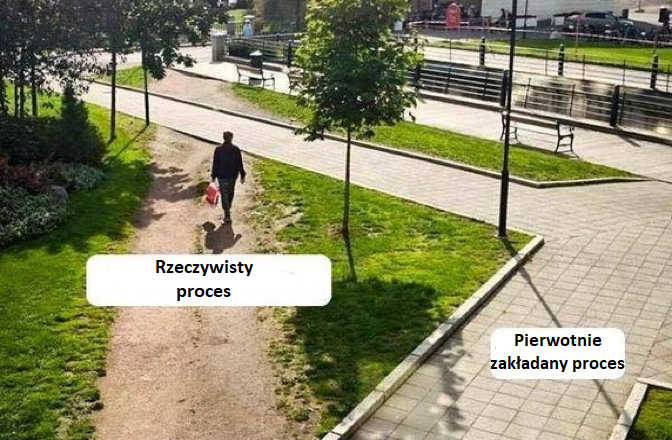
\includegraphics[scale=0.5]{model-vs-real.png}}
	\caption{\label{fig:subcaption_example}Proces rzeczywisty i pierwotnie zakładany}
\end{figure}

\subsection{Algorytmy do wykrywania procesów biznesowych}
Alpha algorithm \newline
The ILP Miner \newline
Heuristic Miner \newline
Multi-phase Miner \newline


%---------------------------------------------------------------------------

\section{Metryki}
\label{sec:metryki}
\cite{doi:10.1142/S0218843014400012}
\subsection{Prostota}
Najprostsza z metryk. \newline
$M_{pro} = 1 - \frac{ilosc\ duplikatow\ w\ modelu\ +\ ilosc\ brakujacych\ wartosci\ w\ modelu}{ilosc\ unikalnych\ zdarzen\ w\ logu\ +\ ilosc\ zdarzen\ w\ modelu}$
\subsection{Odwzorowanie}
Pozostałe metryki obliczane są na podstawie tej metryki. \newline
$M_o = (1 - \sum_{0}^{ilosc\ procesow\ w\ logu} \frac{blad\ odwzorowania\ logu\ w\ modelu}{minimalna\ długosc\ sciezki\ w\ modelu\ +\ długosc\ sciezki\ w\ logu})^4$

Przykład liczenia odwzorowania: \newline

\subsection{Precyzja}

$M_{pre} = (1 - \sum_{0}^{ilosc\ zdarzen\ w\ modelu} \frac{ilosc\ osiagalnych\ zdarzen\ w\ modelu - ilosc\ osiagalnych\ zdarzen\ w\ logu}{ilosc\ osiagalnych\ zdarzen\ w\ modelu})^{\frac{1}{3}} $
\subsection{Generalizacja}
$M_g = \frac{1 - \sum_{0}^{ilosc\ zdarzen\ w\ logu} \frac{1}{\sqrt{ilosc\ wystapien\ zdarzenia}}}{ilosc\ zdarzen\ w\ logu} $
\subsection{Złożoność}
Promuje rozwiązywanie prostych problemów w prosty sposób \newline
$M_z = 1 - \frac{1}{\sqrt{1 - odwzorowanie\ *\ \sqrt{zlozonosc\ modelu}}} $


%---------------------------------------------------------------------------

\section{Ewolucja genetyczna}
\label{sec:ewolucjaGenetyczne}
\subsection{Algorytmy genetyczne}
\cite{ryan_collins_neill_1998}
Algorytmy genetyczne są inspirowaną selekcją naturalną  heurystyką, która używa znanych z ewolucji biologicznej operacji jak mutacja, selekcja czy krzyżowanie do rozwiązywania problemów wyszukiwania i optymizacji. Ich ideą jest zaproponowanie metody przeszukiwania przestrzeni losowy rozwiązań w celu wyszukania najlepszych z nich. Pierwszy raz zostały zaproponowane w \cite{10.5555/138936}.

Sposób działania algorytmów genetyczny polega na stworzeniu populacji losowych rozwiązań zwanych genotypami lub chromosomami, które kodowane są za pomocą licz całkowitych i zapisywane ww tablicy jednowymiarowej. Następnie dla każdego elementu populacji obliczane są metryki pozwalające ocenić jak dobre jest wygenerowane rozwiązanie. Po sklasyfikowaniu rozwiązań generujemy nową populację mutując lub krzyżując głownie choć nie tylko najlepsze chromosomy. Proces ten jest powtarzany do momentu otrzymania satysfakcjonującego rozwiązania.  

Selekcja:
Selekcja proporcjonalna - wybieramy losowo rozwiązania z puli wszystkich rozwiązań z warunkiem, że rozwiązania z największą wartością metryk mają największą szansę na bycie zachowanymi w populacji. Jest to najpopularniejsza metoda selekcji i najczęściej umożliwiająca najszybsze znalezienie rozwiązania. Pozwala na elityzm, czyli zachowanie części najlepszych genotypów w przyszłej populacji.

Selekcja turniejowa - wybieramy podzbiór ze zbioru rozwiązań i zachowujemy w przyszłej najlepsze rozwiązanie z tego podzbioru.
Rozwiązanie to pozwala na duży wpływ na presję genetyczną - zwiększając wielkość podzbioru ograniczamy szansę na wybór z niską wartością metryk.  Jest to także metoda, która łatwe zrównoleglenie.

Krzyżowanie - :
Krzyżowanie punktowe - spośród dwóch genotypów losowo wybieramy jeden punkt, następnie tworzymy dwa nowe genotypy pierwszy z chromosomów na prawo od punktu w pierwszym genotypie i na lewo w genotypie drugim oraz drugi z dwóch pozostałych.

Krzyżowanie dwupunktowe - spośród dwóch genotypów losowo wybieramy dwa punkty, następnie część pomiędzy tymi punktami jest zamieniana pomiędzy genotypami.

Krzyżowanie n-punktowe - uogólnienie powyższych krzyżowań dla n punktów.

Krzyżowanie zamiana w drzewie - genotyp może być reprezentowany jako drzewo, w tej metodzie zamieniamy ze sobą dwa poddrzewa, tworzone są tylko prawidłowe rozwiązania, jednak jest to metoda wymagająca większej ilości obliczeń. 


Mutacja:
Mutacja punkowa - dowolna wartość w tablicy zostaje zmieniona na inną losową wartość. Pozostałe produkcje pozostają niezmienione.

Mutacja zamiana w drzewie - genotyp może być reprezentowany jako drzewo, w tej metodzie tworzone jest nowe poddrzewo, przy tej metodzie tworzone są tylko prawidłowe rozwiązania, jednak jest to metoda wymagająca większej ilości obliczeń. 

 
  
\subsection{Ewolucja genetyczna a inne algorytmy uczenia maszynowego}
Algorytmy genetyczne pozwalają przeszukać najszerszą przestrzeń rozwiązań. Pozwalają na znajdowanie nieoczywistych rozwiązań.  
Inna heurystyką, która używa losowo rozwiązuje problem jest simulated annealing. Algorytm genetyczny jest łatwy w zrównogleniu i pozwala znaleźć globalne rozwiązanie.
Sieci neuronewe:
Pula rozwiązań zamiast jednego rozwiązywania. Szersze przeszukiwanie rozwiązań. 
\subsection{Ewolucja gramatyczna}
Ewoluuje gramatykę za pomocą metod ewolucji genetycznej w celu znalezienia programu, który najlepiej rozwiązuje problem.
Podejście to zostało zaproponowane w \cite{ryan_collins_neill_1998}. 

%---------------------------------------------------------------------------

\section{Gramatyka}
\label{sec:gramatyka}
\subsection{BNF}
Backus-Naur from jest notacją używaną do kodowaniu gramatyk bezkontekstowych.

Gramatyka bezkontekstowa - 

Gramtyka G=(N,$\Sigma$,P,S) - 

\subsection{Tworzenie gramatyki pod kątem ewolucji}

W celu ograniczenia niepotrzebnych obliczeń gramatyka powinna tworzyć jak najmniej niewłaściwych rozwiązań. 
Tworząc gramatykę pod kątem wykorzystania jej w procesie ewolucji ważne jest, żeby ilość produkcji jak najlepiej odzwierciedlała jak często chcemy uzyskać dany stan.
Stosując operator mutacji możemy uzyskać genotypy, które nie należą do języka, czyli nie są właściwym rozwiązaniami. Żeby ograniczyć zbędne obliczenia gramatyka powinna minimalizować szansę na to, że zamieniając produkcję na dowolną inną dostępną dla danego symbolu produkcję uzyskamy słowo które nie należy do języka.
Przykład:
a+b
<e> = aSe | b
<S> = + | -

<e> = aee | b | + | -

Produkcja 1:

<e> -> aSe -> a+e -> a+b
Produkcja 2:
<e> -> aee -> a+e -> a+b

Jeśli w kroku a+e zajdzie mutacja, może uzyskać gramatykę np. a+-, która nie należy do języka, dlatego pierwsza gramatyka jest lepsza.